\documentclass[10pt]{beamer}
\usepackage{amsmath,amssymb,longtable,hhline}
\usepackage{mathrsfs}
\usepackage{xcolor}
\usepackage{hyperref}
\usepackage{multicol}
\usepackage{anyfontsize}
\usepackage{minted}
\usepackage{alltt}

\usemintedstyle{tango}
\newcommand{\ltprgsize}{\fontsize{5}{5}\selectfont}
%\newcommand{\ltprgsize}{\footnotesize}
\setminted{fontsize=\footnotesize,mathescape}

\definecolor{mygreen}{rgb}{0,0.6,0}
\definecolor{mygray}{rgb}{0.5,0.5,0.5}
\definecolor{mymauve}{rgb}{0.58,0,0.82}

\hypersetup{
    bookmarks=true,         % show bookmarks bar?
    unicode=true,           % non-Latin characters in Acrobat’s bookmarks
    pdftoolbar=false,        % show Acrobat’s toolbar?
    pdfmenubar=false,        % show Acrobat’s menu?
    pdffitwindow=false,     % window fit to page when opened
    pdfstartview={FitH},    % fits the width of the page to the window
    pdftitle={},    % title
    pdfauthor={Evgeny Cherkashin},     % author
    pdfsubject={model driven architecture},   % subject of the document
    pdfnewwindow=true,      % links in new PDF window
    colorlinks=true,       % false: boxed links; true: colored links
    linkcolor=red,          % color of internal links (change box color with linkbordercolor)
    citecolor=green,        % color of links to bibliography
    filecolor=magenta,      % color of file links
    urlcolor=blue           % color of external links
}

\usepackage{pifont}

\usetheme{Warsaw}
\usecolortheme{crane}
%\useinnertheme{rectangles}
%\setbeamertemplate{itemize item}{\scriptsize\hbox{\donotcoloroutermaths\ding{113}}}
\definecolor{darkding}{RGB}{200,56,0}
\setbeamertemplate{itemize item}{\scriptsize\hbox{\color{darkding}{\bfseries\ding{113}}}}
\setbeamertemplate{itemize subitem}{\tiny\raise1.5pt\hbox{\donotcoloroutermaths$\blacktriangleright$}}
\setbeamertemplate{itemize subsubitem}{\tiny\raise1.5pt\hbox{\donotcoloroutermaths$\blacktriangleright$}}
\setbeamertemplate{enumerate item}{\insertenumlabel.}
\setbeamertemplate{enumerate subitem}{\insertenumlabel.\insertsubenumlabel}
\setbeamertemplate{enumerate subsubitem}{\insertenumlabel.\insertsubenumlabel.\insertsubsubenumlabel}
\setbeamertemplate{enumerate mini template}{\insertenumlabel}

\beamertemplatenavigationsymbolsempty

\usepackage{iftex,ifxetex}
\ifPDFTeX
  \usepackag
%\useoutertheme{split}
%\useinnertheme{rounded}
\setbeamertemplate{background canvas}[vertical shading][bottom=white!80!cyan!20,top=cyan!10]
%\setbeamertemplate{sidebar canvas left}[horizontal shading][left=white!40!black,right=black]

\graphicspath{{pics/}}

\providecommand{\email}[1]{\texttt{#1}}
\usepackage{changepage}
\newcommand{\GB}[1]{\colorbox{green}{#1}}
\newcommand{\BB}[1]{\colorbox{blue}{#1}}
\newcommand{\RB}[1]{\colorbox{red}{#1}}
\newcommand{\btprgsize}{\fontsize{7}{7}\selectfont}

% --------------------------

\begin{document}

\Setbeamertemplatee[utf8]{inputenc}
  \usepackage[T1]{fontenc}
  \usepackage[russian]{babel}
  \usepackage{lmodern}
  \usefonttheme{serif}
\else
  \ifluatex
    \usepackage{unicode-math}
    \defaultfontfeatures{Ligatures=TeX,Numbers=OldStyle}
    \setmathfont{Latin Modern Math}
    \setsansfont{Linux Biolinum O}
    \setmonofont{Fira Mono}[Scale=MatchLowercase]
    \usefonttheme{professionalfonts}
    % \setmathfont[
    %     Ligatures=TeX,
    %     Scale=MatchLowercase,
    %     math-style=upright,
    %     vargreek-shape=unicode
    %     ]{euler.otf}
  \fi
\fi

%\useoutertheme{split}
%\useinnertheme{rounded}
\setbeamertemplate{background canvas}[vertical shading][bottom=white!80!cyan!20,top=cyan!10]
%\setbeamertemplate{sidebar canvas left}[horizontal shading][left=white!40!black,right=black]

\graphicspath{{pics/}}

\providecommand{\email}[1]{\texttt{#1}}
\usepackage{changepage}
\newcommand{\GB}[1]{\colorbox{green}{#1}}
\newcommand{\BB}[1]{\colorbox{blue}{#1}}
\newcommand{\RB}[1]{\colorbox{red}{#1}}
\newcommand{\btprgsize}{\fontsize{7}{7}\selectfont}

% --------------------------

\begin{document}

\setbeamertemplate{background canvas}[vertical shading][bottom=white,top=white]
\setbeamercolor{background canvas}{bg=white}

\title{Knowledge graph based distributed infrastructure for processing documents used for organizing education process}
\author[E.~Cherkashin]{\bfseries%
  Evgeny A. Cherkashin, Victoria A. Popova}
\institute{\normalsize Matrosov Institute for System Dynamics and Control Theory of Siberian Branch of Russian Academy of Sciences, Irkutsk, Russia\\%
  Institute of Mathematics and Information Technologies, Irkutsk State University, Irkutsk, Russia\\
  \email{\href{mailto:eugeneai@icc.ru}{eugeneai@icc.ru}},\quad \email{\href{mailto:victorypopova1@gmail.com}{victorypopova1@gmail.com}}%
}
\date[2021]{AIIT'2022, October, 14, 2022 \\
Zrenjanin, Serbia}
%\date{\today}
\maketitle

\begin{frame}
\frametitle{Research and Development objectives}
Irkutsk state university (ISU) has quite normal (required) level of automation in the areas of
\begin{itemize}
\item accounting (``1C:Accounting for budget institutions''),
\item education process planning (``1C:University''),
\item learning management, student state control (``Moodle'')
\item library data access with library information system (LMS ``Irbis-64'').
\end{itemize}
\textbf{BUT} other problems' automation has an \textbf{island character}.
\begin{itemize}
\item institutes of ISU develop software for local purposes,
\item do not share results between ISU community;
\item some solutions are implemented by a subdepartment IMIT of ISU on a request.
\end{itemize}
\textbf{Main objective} of the present research  is to creative activities of the faculty
\begin{itemize}
\item authoring syllabi,
\item organizing processes, monitoring and control,
\item form a basis of educational process modeling to support the
  \begin{itemize}
  \item ministry requirements compliance checking,
  \item compliance to domain of courses,
  \item individual education trajectories of students.
  \end{itemize}
\end{itemize}
\end{frame}

\begin{frame}
\frametitle{Syllabi authoring}
One of the challenging problem is course documentation, such as syllabi, mediation the previous version with the current curriculum.  For a syllabi, following steps are to be performed:
\begin{enumerate}
\item Find a syllabus source at user's PC,
\item Analyze actual curriculum, and find education unit (EU) distribution data, print/write it down,
\item Recall the scenario of course teaching, add/remove/\textbf{comment} topics and laboratory work (LW) task set,
\item Reconcile topics LW with exams question set an the set of competence,
\item Fill in the results in the current template, upload \textbf{DOCX} to institute's cloud storage.
\end{enumerate}

As faculty varies, set of courses varies, EU distribution varies, \ldots, sources lost. We have to do with this!

\textbf{Long term result is} a model of the education process.
\end{frame}

\begin{frame}
  \frametitle{Schedule compilation and student progress monitoring}
  Class scheduling and student progress monitoring have many aspects of consideration,
  \begin{itemize}
  \item a classic combinatorial optimization constraint satisfaction problem,
  \item integration with education process planning software (``1C:University''),
  \item Reconciling with other institutions occupying the same resources,
  \item Accounting faculty requests and students' load,
  \end{itemize}
\vfil
  \textbf{Long term result is} a model of the education process.

  % Data representation for students'
  % \begin{itemize}
  %   \item grades (formal and instructive),
  %   \item compliance to educational trajectories, competence set,
  %   \item creative solutions, and
  %   \item formal tests.
  % \end{itemize}
\end{frame}

\begin{frame}
  \frametitle{Assets, requirements}
  The problem set
  \begin{itemize}
  \item Syllabi published on ISU web site for the active students' groups,
  \item Educational, industrial standards on the government site (some of them just image scans),
  \item Document templates produced by institute management staff,
  \item Data of the developed applications.
  \end{itemize}
  So, at the firs stages we deal with information acquisition and analysis to reach a reasonable level of formalization.  This results to the following general requirements:
  \begin{enumerate}
  \item Allow loose coupling between application (agents) and independent development,
  \item Store data with metadata to form a standardized level of application interaction,
  \item Respect users' day-to-day way of task solution (principle of least surprise),
  \item Use perspective information technologies.
  \end{enumerate}

\end{frame}

\begin{frame}[fragile]\frametitle{Architecture of the infrastructure}
  \begin{columns}
    \begin{column}{0.7\linewidth}
      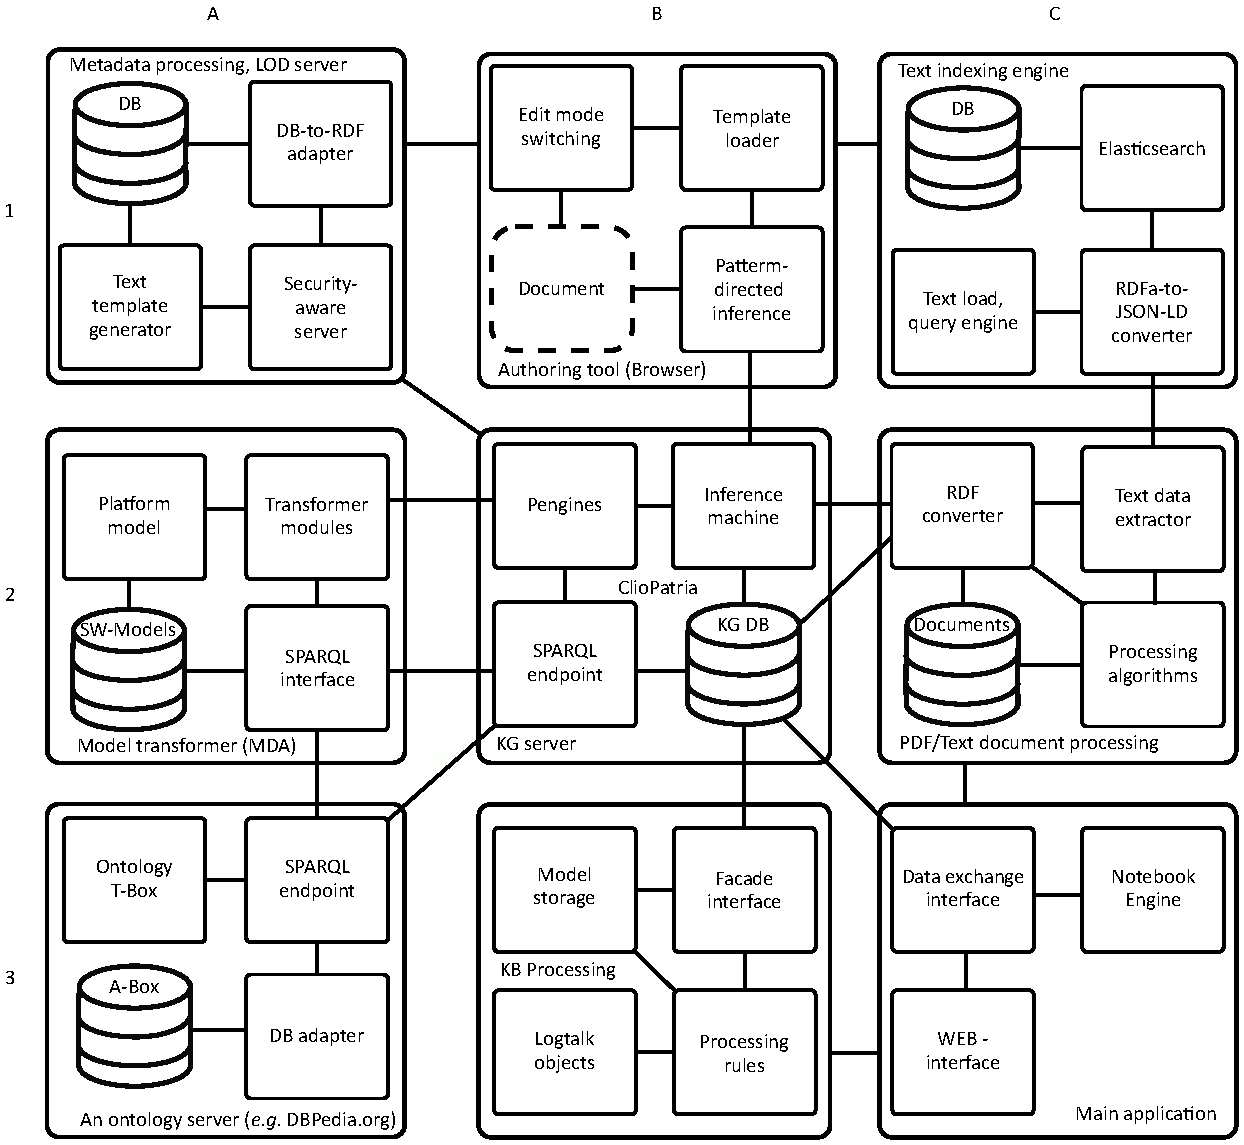
\includegraphics[width=1\linewidth]{architecture-mda-lod-ext-general.pdf}
    \end{column}
    \begin{column}{0.3\linewidth}
      \textbf{Abbreviations}\\[1ex]\scriptsize
      T-Module is Transformation module\\
      MDA is Model-Driven Architecture\\
      % CIM is Computationally Independent Model\\
      % PIM is Platform Independent Model\\
      % PSM is Platform Specific Model\\
      T-Box is Terminological Box\\
      A-Box is Instance Box\\
      % NGS is Next-Generation Sequencing\\
      KG DB is Knowledge Graph Database
    \end{column}
  \end{columns}
\end{frame}

\begin{frame}[fragile]
  \frametitle{Semantic web technologies \& Knowledge graphs}
  Semantic Web (WEB 3.0) is characterized with
  \begin{itemize}
  \item Technological basis, oriented to the web % User applications are always comprises interconnected distributed web-services.
  \item Standardized data formats, storage, and processing
  \item Open principles of data publishing
  % \item Knowledge Graph (KG) construction techniques
  \item Services for data storage and access provision
  \item Generalized and special user interfaces are used for data presentation\vspace{1em}
  \end{itemize}
%\end{frame}

% Knowledge graphs changed the aspects to the knowledge base as being a part of whole totality of knowledge, implying the obeying the global standards and techniques of its acquisition and processing.

%\begin{frame}
%  \frametitle{Knowledge Graphs}
For the Knowledge Graphs (KG), the following is of interest.
 \begin{itemize}
  \item Converged notions \textbf{data} and \textbf{knowledge} as something is \textbf{known}
  \item Contain data, relations, and metadata (vocabularies)
  \item Distinguished \textbf{node filling in} and \textbf{processing} graph triples, \emph{e.g.}, with SPARQL queries with UPDATEs
  \item Allow \textbf{postpone} the formal definition of a schema
  \item Three types of graph schemata: \textbf{semantic} (aimed at generalization), \textbf{validating} (\textbf{e.g.} semantics, \textbf{completeness} w.r.t. sets of relations), and \textbf{emergent} (infer a set of generalized structures and \textbf{reconstruct} the KG).
  \end{itemize}
\end{frame}

\begin{frame}[fragile]
  \frametitle{Logtalk Categories PLACEHOLDER}
  A category of named entities
\begin{minted}[fontsize=\scriptsize]{logtalk}
:- category(named).
:- public([name/1, render/1]).
:- protected([renderitem/2]).
name(Name):- ::prepend(name(Name)).
renderitem(name(Name), String):-!, atom_string(Name, String).
render(String):-  % What is code generation from items
    ::item(name(Name)), ::renderitem(name(Name), String).
:-end_category.
\end{minted}
Category of named and typed entities
\begin{minted}[fontsize=\scriptsize]{logtalk}
:- category(namedtyped, extends(named)).
:- public([type/1,render/2, separator_option/2,list_separator/1]).
:- protected([renderitem/2]).
type(Type):- ::append(type(Type)).
renderitem(Item, String):- ^^renderitem(Item, String),!.
renderitem(type(Type),String):-!, ::list_separator(Separator),
    writef::swritef(String, '%w%w', [Separator, Type]).
render(Middle, String):- ^^render(SName),
    (   ::item(type(Type)) ->
        ::renderitem(type(Type), SType),
        string_concat(SName, Middle, _1),
        string_concat(_1, SType, String) ;
        SName = String  ).
render(String):-  ::render("", String).
list_separator(Separator):-
    ::separator_option(Name, Default),!, % Global options
    root::option(Name, Separator, Default).
:- end_category.

\end{minted}
\end{frame}




\begin{frame}
  \frametitle{Conclusion}
  This is a progress report of R\&D of a Knowledge Graph based architecture and infrastructure for automation of creative activity of a faculty.  The following results were obtained:
  \begin{enumerate}
  \item Raw domain analysis, including, problem space,
  \item Existing software and data source accounting,
  \item Realized MVP-like utilities providing solutions of new problems
    \begin{itemize}
    \item Knowledge Graph (KG) component infrastructure is being organized,
    \item Analyzing PDF-exported versions of syllabi by a Logtalk knowledge-based system,
    \item Collecting data from the syllabi documents an store in KG,
    \item Implementing verification software for parts of a syllabi,
    \item Document authoring tools are being implemented using generative approaches,
    \item Techniques of Linked Open Data and standard vocabularies usage is being formalized.
    \end{itemize}
  \end{enumerate}
\end{frame}

\begin{frame}
  \begin{center}
  \Large Thanks for Your Attention!
\end{center}
\end{frame}




\end{document}

%%% Local Variables:
%%% mode: latex
%%% TeX-master: t
%%% End:
